\documentclass{beamer}
\usepackage{beamerthemesplit} % new 
\usepackage[utf8]{inputenc}
\usetheme{Warsaw}
\begin{document}
\title{Technologies mobiles} 
\author{Olivier Levitt} 
\date{\today} 
\AtBeginSubsection[]
{
  \begin{frame}
  \frametitle{Contents}
  \tiny{\tableofcontents[currentsubsection]}
  \end{frame}
}


\frame{
\titlepage

\includegraphics[width=60pt]{google-android.jpg}

\includegraphics[width=60pt]{ios.png}

\includegraphics[width=60pt]{wp8.jpg}

\includegraphics[width=60pt]{bb10.jpg}
} 

\frame{\frametitle{Sommaire}\tableofcontents} 
 
\section{Présentation et objectifs du cours}
\subsection{Organisation administrative}
\frame{
\frametitle{Planning}
\begin{itemize}
  \item{30 janvier : 3h de cours, 3h de TP}
  \item{6 février : 3h de cours}
  \item{13 février : 6h de TP}
  \item{Validation des sujets de projet avant le 20 février}
  \item{20 février : 6h de TP dédiées au projet}
  \item {? mars : Soutenance du projet}
\end{itemize}
}
\frame{
\frametitle{Evaluation}
\begin{itemize}
  \item{Projet : création d'une application}
  \item{Groupe de 2}
  \item{Sujet ``libre''}
  \item{6h de TP dédiées au projet + travail personnel}
  \item{Soutenance / Présentation de l'application}
\end{itemize}
}
\subsection{Champ du cours}
\frame{
\frametitle{Contexte}
\begin{itemize}
  \item Smartphones, tablettes et assimilés (TV, montre, autoradio \ldots)
  \item Dev d'application, pas de dev de la plateforme
  \item 1ère partie : le dev mobile en général
  \item 2ème partie : application sous android
\end{itemize}
}

\section{Le développement mobile} 
\subsection{Spécificités du développement mobile}
\frame{
\frametitle{Des appareils suréquipés}
\begin{itemize}
  \item Téléphonie (SMS, MMS, appels)
  \item Internet (GPRS, EDGE, 3G, 4G, WIFI)
  \item Réseaux locaux (Bluetooth, réseaux adhoc, NFC)
  \item Capteurs (Luminosité, proximité)
  \item Localisation (GPS, triangulation, SSID wifi)
  \item Notifications (Vibreur, haut-parleurs, LED)
  \item Stockage de données (Mémoire flash, SD externe, SQLite)
  \item Interactions (Ecran tactile, gestures, boutons physique)
  \item Et encore d'autres \ldots
\end{itemize}
Et des API pour utiliser tout ça !
}
\frame{
\frametitle{Des contraintes techniques importantes}
\begin{itemize}
  \item Processeur
  \item Mémoire RAM
  \item Stockage de données
  \item Gestion de la batterie
  \item Stabilité et débit de la connexion internet
  \item Cycle de vie de l'application
  \item Taille d'écran 
  \item Inputs atypiques (clavier virtuel, gestures, peu de boutons \ldots)
\end{itemize}
Contraintes à garder en tête en permanence.
}
\frame{
\frametitle{La fragmentation}
Une application publiée sur le google playstore cible plus de 2400 appareils
différents !\\
\begin{itemize}
   \item ``Write once, run everywhere'' ?
   \item Comment tester / débugger pour tous ces appareils ?
  \item Eviter de géner l'utilisateur (versions HD, appareils non compatibles)
  \item S'adapter quand une fonctionnalité n'est pas disponible
\end{itemize}
}
\frame{
\frametitle{La fragmentation, taille d'écran}
Comment gérer toutes les tailles d'écran ? 
\begin{itemize}
  \item Montres connéctées : de 1 à 2 pouces
  \item Smartphones lowcost : 3 pouces (Galaxy pocket, galaxy Y)
  \item Smartphones high-end : 4 à 5 pouces (IPhone 5, HTC 8X, nexus 4)
  \item Phablets : 5 à 6 pouces (Galaxy note, HTC butterfly)
  \item Tablettes : 7 pouces (Nexus 7, IPad mini), 8 pouces (Archos 80g9), 10 pouces (Nexus 10, IPad)
\end{itemize}
}


\frame{
\frametitle{De nombreuses autres sources de fragmentation}
\begin{itemize}
  \item Versions de l'OS
  \item Résolutions d'écran
  \item Elements hardware présents
  \item Puissance
  \item Modifications constructeur / ``rom custom''
  \item \ldots
\end{itemize}
}
\frame{
\frametitle{Des Ecosystèmes forts}
\begin{itemize}
  \item Obligation d'utiliser le SDK fourni
  \item Suivre les guidelines
  \item Restrictions liées à la plateforme
  \item Utilisation des services de la plateforme
  \item Processus de déploiement des applications
  \item Règles des ``store'' (validation, monétisation \ldots)
\end{itemize}
}
\subsection{Comparaison des différents OS mobile}

\section{Le développement sur android} 

\subsection{Mise en place}
\frame{
\frametitle{Les marque-page}
\begin{itemize}
  \item www.frandroid.com (actu FR)
  \item www.androidpolice.com (actu EN)
  \item www.androidcentral.com (actu EN)
  \item www.d.android.com (la bible EN)
  \item www.stackoverflow (Q/A EN)
  \item \#android et \#android-dev sur freenode (chat irc EN)
  \item www.breizhjug.org et www.paug.fr (communautés FR)
  \item www.google.fr (réservoir à tutoriels)
\end{itemize}
}
\frame{
\frametitle{Bien commencer}
La programmation android fait partie des plus accessibles :
\begin{itemize}
  \item Des (bonnes) bases de programmation en JAVA
  \item Un ordinateur (Windows, Linux, Mac OS X)
  \item Un appareil android (conseillé, l'émulateur étant \ldots moyen)
\end{itemize}
C'est tout !
}
\frame{
\frametitle{Les niveaux d'API}
\begin{table}
\begin{tabular}{|l|c|c|c|r|}
  \hline
  Version & Nom & API level & Distribution & Cumulé \\
  \hline
  1.5 & Cupcake & 3 & 0\% & 0\% \\
  1.6 & Donut & 4 & 0.2\% & 0.2\% \\
  2.1 & Eclair & 7 & 2.4\% & 2.6\% \\
  2.2 & Froyo & 8 & 9\% & 11.6\% \\
  2.3 & Gingerbread & 9/10 & 47.6\% & 59.2\% \\
  3.X & Honeycomb & 12/13 & 1.5\% & 60.7\% \\
  4.0.X & Ice cream sandwich & 15 & 29.1\% & 89.8\% \\
  4.1 & Jelly bean & 16 & 9\% & 98.8\% \\
  4.2 & Jelly bean & 17 & 1.2\% & 100\% \\
  \hline
\end{tabular}
\caption{\label{s}Répartition des versions pour les accès au google play sur la
dernière quinzaine de 2012}
\end{table}
}
\frame{
\frametitle{Présentation du SDK android}
Téléchargement gratuit : www.d.android.com/sdk
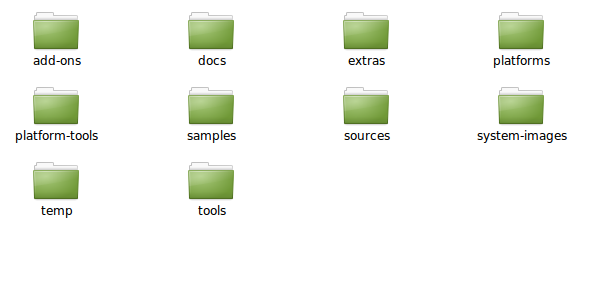
\includegraphics[width=300pt]{sdk.png}
}
\frame{
\frametitle{Présentation du SDK android}
\begin{itemize}
  \item add-ons : Google APIs
  \item docs : Copie de la documentation disponible sur d.android.com
  \item extras : Lib de compatibilité, lib pour les achats in-app \ldots
  \item platform-tools : Binaires de communication avec les appareils android
  (adb, fastboot \ldots)
  \item platforms : 1 dossier par niveau d'API téléchargé
  \item samples : Exemples de projets
  \item sources : Sources de chaque niveau d'API
  \item system-images : Images pour l'émulateur
  \item temp
  \item tools : Outils pour le dev (ddms, apkbuilder, lint \ldots)
\end{itemize}
}
\frame{
\frametitle{Plugin android pour eclipse : ADT}
Installation comme un plugin eclipse classique\\ 
https://dl-ssl.google.com/android/eclipse/\\
ADT fait le lien entre eclipse et le SDK android
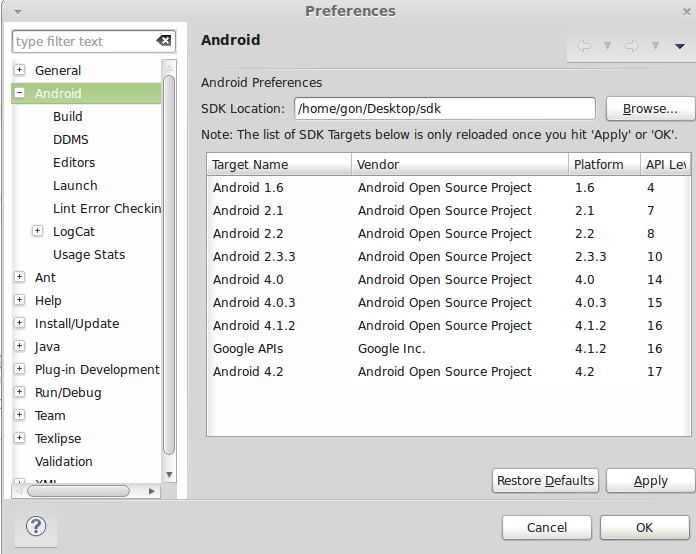
\includegraphics[width=100pt]{adt.png}
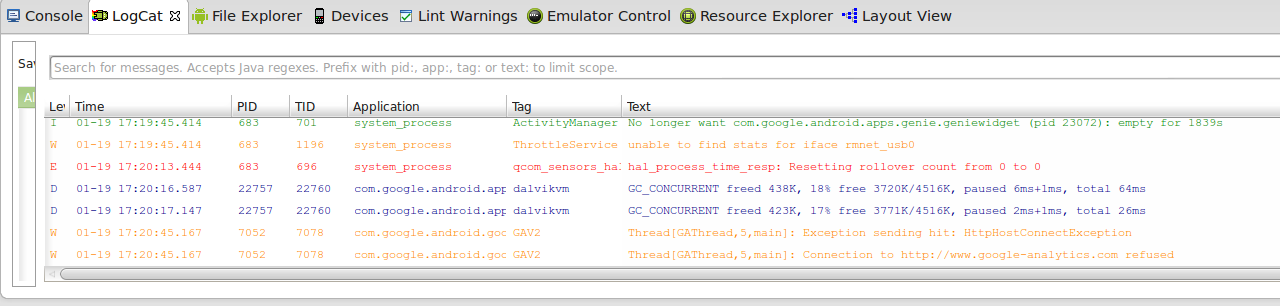
\includegraphics[width=200pt]{views.png}\\\\
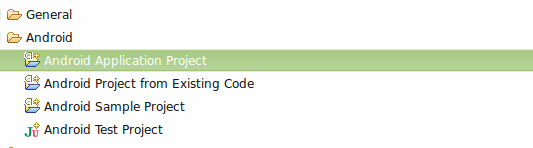
\includegraphics[width=100pt]{project.png}
}
\frame{
\frametitle{L'émulateur}
\begin{itemize}
  \item Utile pour tester certaines configurations
  \item ((très) (très)) lent
  \item Utiliser un appareil android à la place quand c'est possible
\end{itemize}
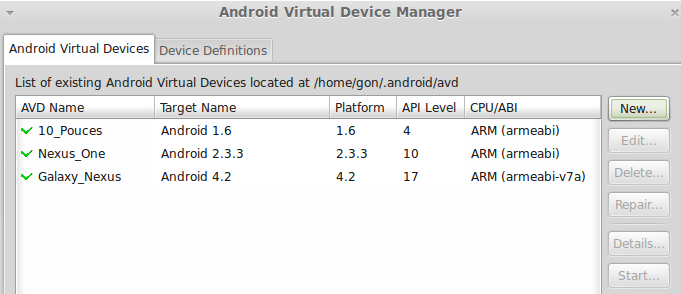
\includegraphics[width=300pt]{avd.png}
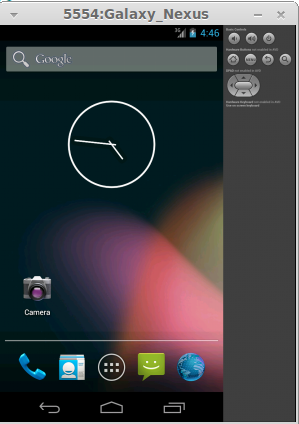
\includegraphics[width=42pt]{emu.png}
}
\frame{
\frametitle{Alternative à l'émulateur}
\begin{itemize}
  \item Problème : émuler de l'ARM sur nos machines x86
  \item Résultat : émulateur (très (très)) lent
  \item Solution proposée : porter android sur x86
  \item http://www.android-x86.org/
\end{itemize}
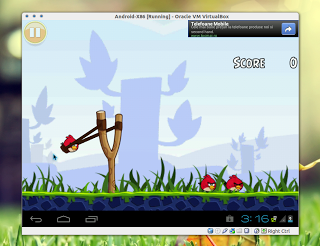
\includegraphics[width=170pt]{x86.png}
}
\frame{
\frametitle{Distribuer l'application}
\begin{itemize}
  \item Une application android = un APK (+/- équivalent d'un jar)
  \item Création et signature de l'APK simple sous eclipse
  \item Distribution directe de l'APK (ex : pour tester, béta fermée)
  \item Publication sur le playstore, 25\$ à l'inscription
  \item Application gratuite ou payante (30\% pour google)
 \end{itemize}
}
\subsection{Architecture}
\frame{
\frametitle{Organisation d'un projet android}
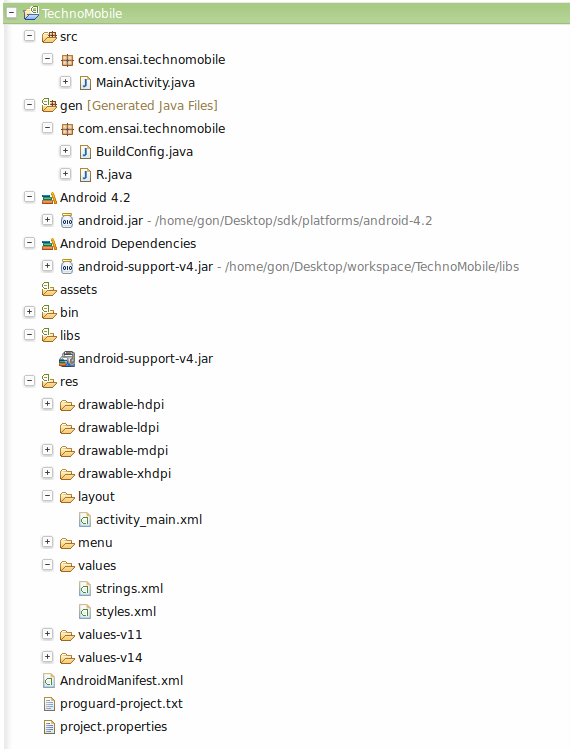
\includegraphics[width=150pt]{structure.png}
}
\frame{
\frametitle{Détail de l'organisation}
\begin{itemize}
  \item src : code source java
  \item gen : identifiants des ressources (généré par le sdk)
  \item Android 4.2 : jar correspondant à l'API cible
  \item Android Dependencies : jar rajoutés, correspond à libs
  \item assets : fichiers fournis avec l'app
  \item bin : résultat de la compilation (dont l'apk)
  \item libs : jar rajoutés
  \item res : ressources (layouts, strings, images \ldots)
  \item AndroidManifest.xml : métadonnées sur l'application, composants,
  permissions \ldots
  \item proguard-project.txt : configuration de proguard
  \item project.properties : généré par le sdk
 \end{itemize}
}
\frame{
\frametitle{AndroidManifest.xml : le coeur de l'application}
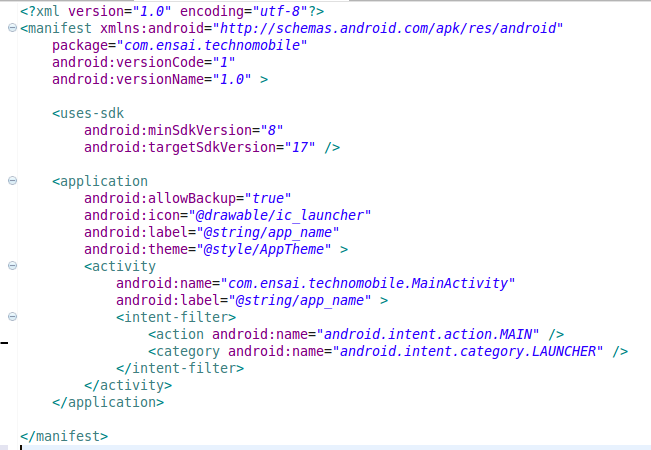
\includegraphics[width=150pt]{manifest.png}
}
\frame{
\frametitle{Activity et cycle de vie de l'application}
}
\subsection{IHM}
\subsection{Données}




\end{document}
